\subsection*{Hardware Software co-design}
\underline{Loop unrolling:}\\
Loop unrolling consits of replicating the body of a loop to reduce the number of iterations.

\begin{minipage}{0.69\columnwidth}
    \begin{minted}{c}
for (i = 0; i < 3; i++) {
    for (j = 0; j < 3; j++) {
        a[i][j] = 0;
    }
}
\end{minted}
\end{minipage}
%\hfill
$\Longleftrightarrow $
\begin{minipage}{0.29\columnwidth}
    \begin{minted}{c}
a[0][0] = 0;
a[0][1] = 0;
a[0][2] = 0;
a[1][0] = 0;
a[1][1] = 0;
a[1][2] = 0;
a[2][0] = 0;
a[2][1] = 0;
a[2][2] = 0;
\end{minted}
\end{minipage}

\underline{In-lining:}\\
In-lining consists of replacing a function call by the body of the function.
The keyword \texttt{inline} can also be used to force the compiler to inline a function.
The compiler option \texttt{-O3} enables in-lining.

\begin{minipage}{0.49\columnwidth}
    \begin{minted}{c}
int sum(int a, int b) {
    return a + b;
}
int main() {
    int a = 1;
    int b = 2;
    int c = sum(a, b);
    return 0;
}
\end{minted}
\end{minipage}
%\hfill
$\Longleftrightarrow $
\begin{minipage}{0.49\columnwidth}
    \begin{minted}{c}
int main() {
    int a = 1;
    int b = 2;
    int c = a + b;
    return 0;
}
\end{minted}
\end{minipage}
\underline{Using bit shift instead of multiplication/division:}\\
Multiplication and division are very expensive operations in terms of clock cycles.
It is therefore preferable to use bit shift when possible.

\begin{minipage}{0.49\columnwidth}
    \begin{minted}{c}
int main() {
    int a = 1;
    int b = 2;
    int c = a * b;
    return 0;
}
\end{minted}
\end{minipage}
%\hfill
$\Longleftrightarrow $
\begin{minipage}{0.49\columnwidth}
    \begin{minted}{c}
int main() {
    int a = 1;
    int b = 2;
    int c = a << 1;
    return 0;
}
\end{minted}
\end{minipage}
\underline{Computing inside the return statement:}\\

\begin{minipage}{0.49\columnwidth}
    \begin{minted}{c}
int main() {
    int a = 1;
    int b = 2;
    int c = a + b;
    return c;
}
\end{minted}
\end{minipage}
%\hfill
$\Longleftrightarrow $
\begin{minipage}{0.49\columnwidth}
    \begin{minted}{c}
int main() {
    int a = 1;
    int b = 2;
    return a + b;
}
\end{minted}
\end{minipage}

\underline{Eviter les accès mémoire:}

Par exemple rajouter des variables \texttt{*source} et \texttt{*dest} pour éviter les accès mémoire.

\begin{minipage}{0.49\columnwidth}
    \begin{minted}{c}
int r,g,b;
int x,y,index;
for (y = 0; y < 480; y++) {
    for (x = 0; x < 640; x++) {
        index = y * 640 + x;
        r = source[index];
        g = source[index + 1];
        b = source[index + 2];
    }
}
\end{minted}
\end{minipage}
$\Longleftrightarrow $
\begin{minipage}{0.49\columnwidth}
    \begin{minted}{c}
int r,g,b;
int x,y,index;
int *source;
int *dest;
for (y = 0; y < 480; y++) {
    for (x = 0; x < 640; x++) {
        index = y * 640 + x;
        r = *source++;
        g = *source++;
        b = *source++;
    }
}
\end{minted}
\end{minipage}

\columnbreak

\underline{Trade-off}

On peut remplacer certains bouts de code par du hardware en utilisant des
custom instructions.

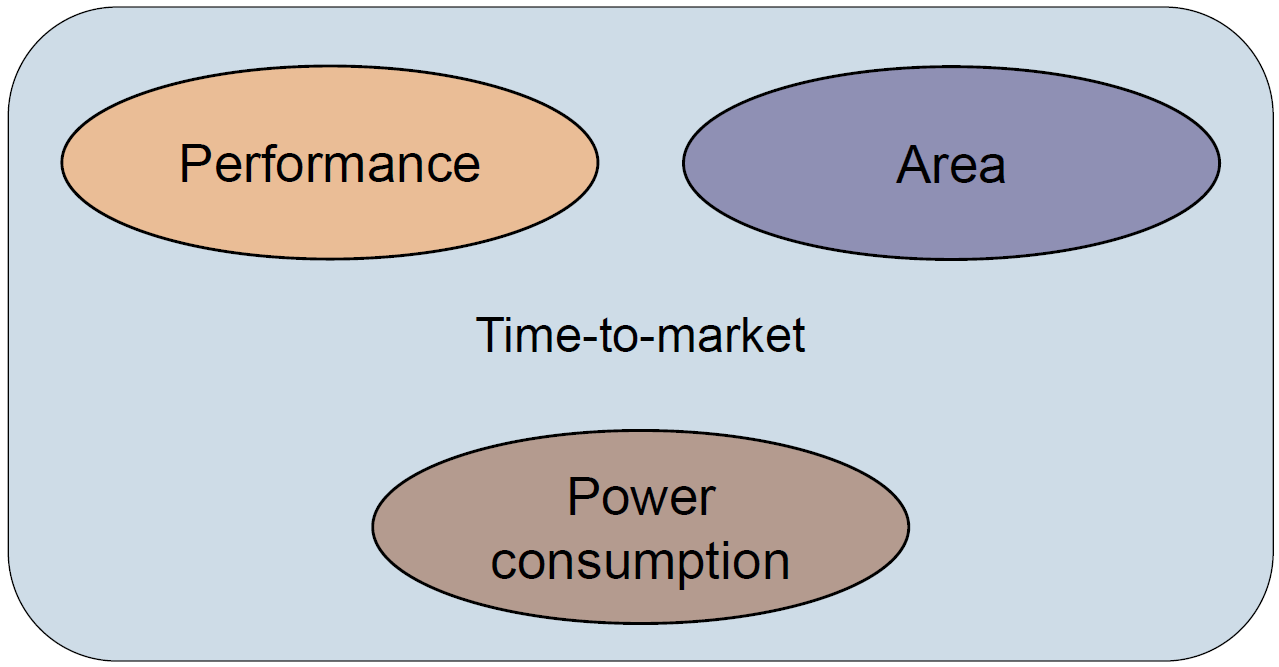
\includegraphics[width=\columnwidth]{images/trade_off_power_area_perf.png}
Facteurs limitants:
\begin{enumerate}[topsep=0pt, partopsep=0pt, itemsep=0pt, parsep=0pt]
    \item Compléxité de l'algorithme à remplacer
    \item Dispoinibilité de ressources hardware
    \item Temps de développement
\end{enumerate}
Avantages:
\begin{enumerate}[topsep=0pt, partopsep=0pt, itemsep=0pt, parsep=0pt]
    \item Performance accrue
    \item Consomation réduite
\end{enumerate}

\underline{Cache:}

Stocke les données les plus utilisées dans un espace mémoire plus rapide.

\underline{Scratchpad:}
Mémoire qui stock les données temporaires du processeur.

\underline{Problème de cohérence:}
Quand deux ou plusieurs processeurs essayent d'accéder à la même donnée en même temps.
Résultats imprévisibles.

MSI (Modified, Shared, Invalid) est un protocole de cohérence de cache.

Mutex: permet de bloquer l'accès à une ressource partagée.

\underline{Profiling:}
Méthode pour analyser les performances d'un programme. Avec un timer on compte le nombre
de cycles d'exécution d'une fonction. Il faut que le timer soit plus rapide que la fonction
qu'on étudie et il faut un timer hardware.


